% Chapter 3

\chapter{Results} % Main chapter title

This section categorizes all results in three parts: neuronal activity simulations, BOLD activity simulations and comparison of brain graphs to randomly constructed graphs. FHN model simulated brain graphs of FCM and ACM are compared to fMRI-BOLD data and DW-MRI data, respectively. Baloon-Windkessel model applied brain graphs of FCM and ACM are compared to single empirical brain map, the fMRI-BOLD data. Random graphs are simulated only with FHN model. The last part aims to illustrate whether these random graphs can be distinguished from brain graphs in terms of the modeled neuronal activity.  

The comparison of simulated brain graphs $s$ to the empirical connectivity matrices $e$ is done statistically via Pearson's correlation coefficient $\rho_{e,s}$. All correlation values are then presented in parameter space for $(r,v)$ and $(r,c)$. Once the most promising simulation is captured, the simulated activity of pairs of nodes are illustrated, i.e. well correlating nodes and bad correlating nodes. The correlation $\rho_{i,j}$ between the simulated activity  of nodes $i$ and $j$ is, 

\begin{equation}
\rho_{i,j} = \dfrac{\big \langle u_i(t) u_{j}(t) \big \rangle - \big \langle u_{i}(t) \big \rangle  \big \langle u_{j}(t) \big \rangle}{ \sigma (u_i(t)) \sigma (u_j(t))}
\end{equation}

where $\sigma$ stands for standard deviation.

Questioning the analogy between random and brain graphs requires another statistical approach then Pearson's analysis, since both graph types are not identical in terms of their network topology. The new strategy is to obtain a histogram for each graph, which represents the distribution of correlation values between nodes after simulations. The degree of similarity between a brain graph histogram $H_{r}$ and random graph histogram $H_{b}$ is calculated via Bhattacharya coefficient \citep{XYZ43},
\begin{equation}
d(H_r, H_b) = \sqrt{1- \dfrac{1}{ \sqrt{\bar{H_r} \bar{H_b} N^2}} \sum_{i} \sqrt{H_r(i)H_b(i)} }
\end{equation}
where $\bar{H}$ denotes the average of histogram. Both $\rho_{e,s}$ and $d(H_r, H_b)$ lie between 0 and 1, however, their interpretation is different. High $\rho_{e,s}$ values presents high correlation, whereas high $d(H_r, H_b)$ points out less similarity. 

\label{Chapter3} % For referencing the chapter elsewhere, use \ref{Chapter1} 

\lhead{Chapter 3. \emph{Results}} % This is for the header on each page - perhaps a shortened title

%----------------------------------------------------------------------------------------

\section{Neuronal Activity Simulations}

\subsection{FCM Brain Graphs Compared to fMRI-BOLD Data}

All brain graphs based on FCM are obtained by binarizing fMRI-BOLD data with threshold values $r$ between $[0.54, 0.66]$. Here, $r$ range corresponds to a network density $D$ approximately between 0.4 and 0.1. Each brain network is then simulated with FHN model, and compared to its empirical data set via Pearson's correlation coefficient, $\rho_{e,s}$. This section begins from a broad manner by demonstrating all $\rho_{e,s}$ values in parameter spaces, and goes narrower into nodal dynamics. 

\begin{figure}[htbp]
 
  \centering
    \includegraphics[width=0.49\textwidth]{Figures/PA_FCM_c_02.eps} 
	\includegraphics[width=0.49\textwidth]{Figures/PA_FCM_v_7.eps} 

	
    \rule{35em}{0.5pt}
  \caption[Parameter Analysis, FCM]{Analogy between FHN simulated FCM brain graphs in parameter spaces $(v,r)$ (constant $c=0.2$, on the left) and $(c,r)$ (constant $v=7[m/s]$ on the right). The colorbars stand for $\rho_{e,s}$.   }
  \label{fig:Parameter Analysis, FCM}
 	
\end{figure}  

Each color coded square in Figure 3.1 corresponds to one $\rho_{e,s}$. Hot colors represent well correlation between simulated and empirical data, 0 means no correlation at all and cold colors below zero points out anti-correlations. It can be inferred that fast signal propagation velocity $v$ above $6 [m/s]$, a low $r$ below $0.61$ and a coupling strength $c$ around $[0.1, 0.4]$ would result in high correlations between simulated and empirical data sets.    

Figure 3.2 illustrates correlation matrices of simulated neuronal activity and fMRI-BOLD, parameters for the simulated activity are decided with the help of Figure 3.1. Each colored square represents whether any pair of nodes $i$ and $j$ addressed on x and y axes are analogous in terms of their temporal dynamics. Colorbar denotes $\rho_{i,j}$ values.

Figure 3.3 exhibits excitatory FHN dynamics for pairs of nodes chosen from Figure 3.2, i.e. well correlating nodes signified with hot color and poorly correlating nodes around green color. Anti-correlating temporal dynamics are not visualized. 


\begin{figure}[htbp]
 
  \centering
	 \includegraphics[width=0.49\textwidth]{Figures/cor_FCM_sim.eps} 
   	 \includegraphics[width=0.49\textwidth]{Figures/cor_FCM_exp.eps} 

    \rule{35em}{0.5pt}
  \caption[High correlated FHN simulation, FCM]{ FHN model simulated FCM graph (on the left) and empirical fMRI-BOLD (on the right) correlation matrices. The parameters for extracted timeseries are $c=0.2$, $v=7 [m/s]$, $r=0.60$, overall correlation between two matrices is $\rho_{e,s} = 0.43$}
      \label{fig:High correlated FHN simulation, FCM}
 	
\end{figure}  



\begin{figure}[htbp]
 
  \centering
	 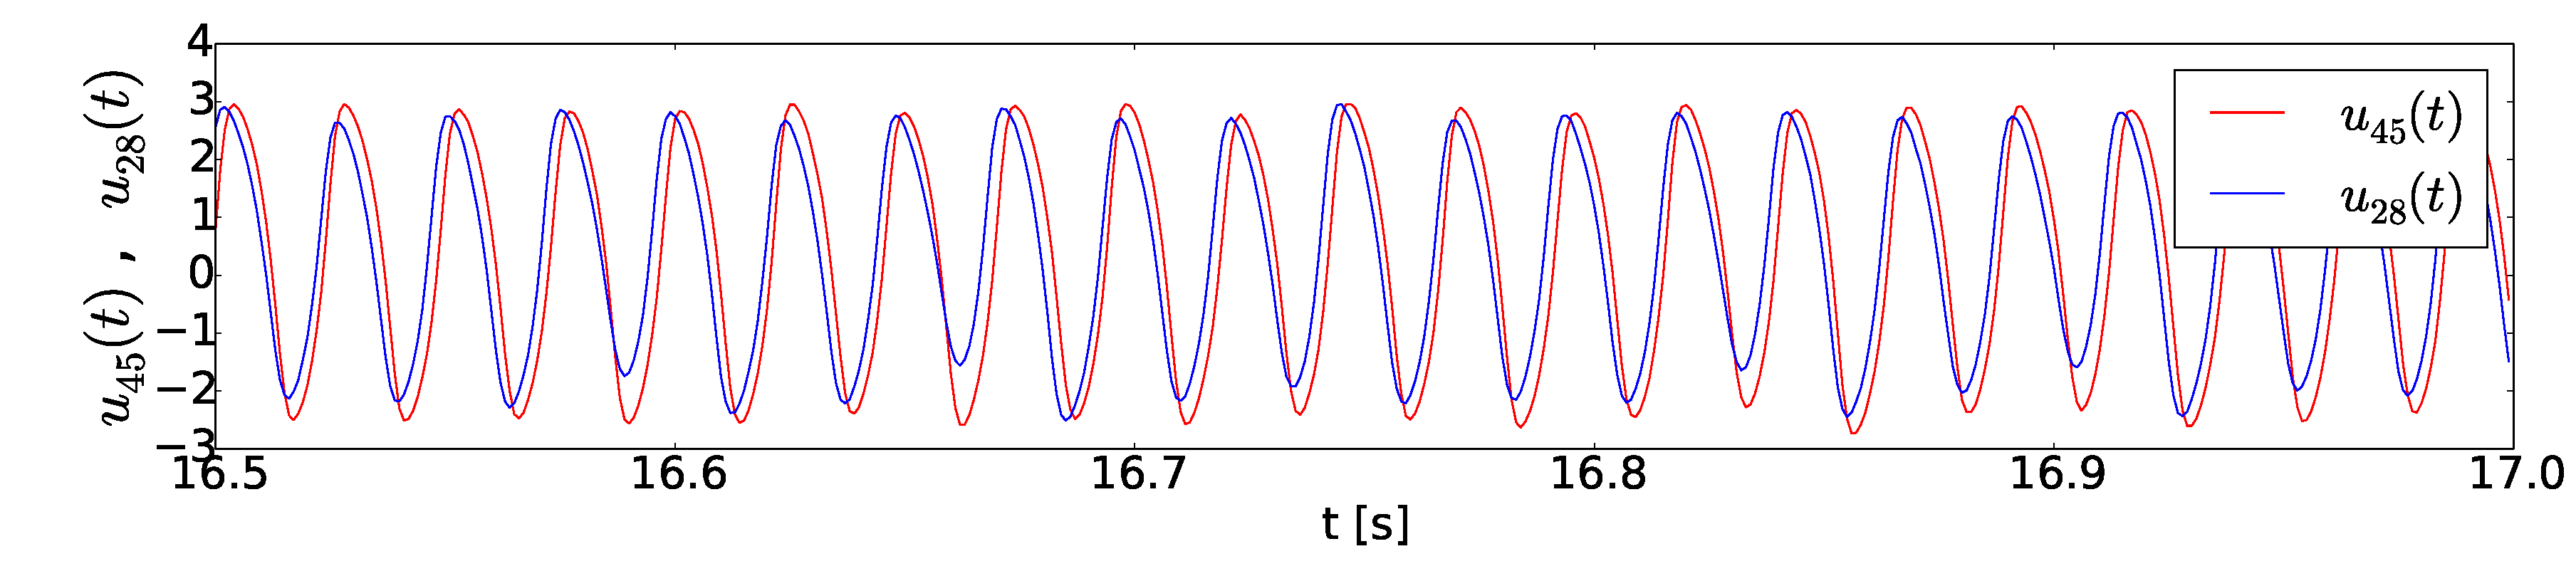
\includegraphics[width=\textwidth]{Figures/cor_FCM_sim_no_best.eps} 
   	 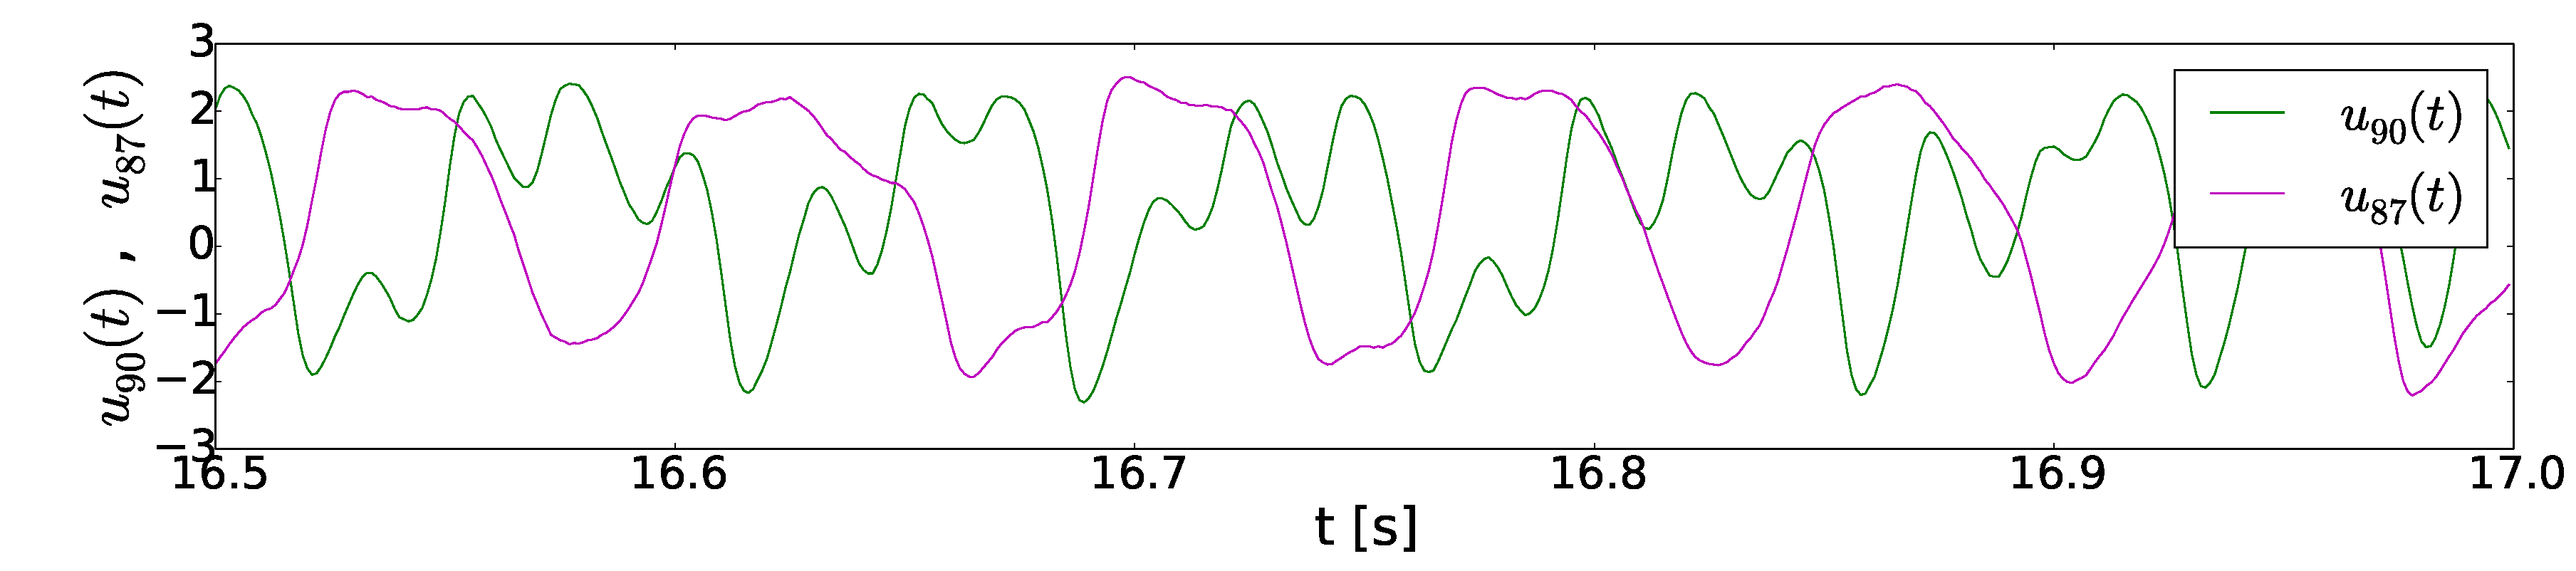
\includegraphics[width=\textwidth]{Figures/cor_FCM_sim_no_worst.eps} 

    \rule{35em}{0.5pt}
  \caption[Neural Activity Node Dynamics, FCM]{Temporal dynamics of highly (at top, $\rho_{45,28}=0.88$) and poorly (at bottom, $\rho_{90,87}=0.13$) correlated node couples with FHN model. Both nodes are chosen from the simulated correlation matrix of FCM in previous figure ($c=0.2$, $v=7 [m/s]$, $r=0.60$).} 
    \label{fig:Neural Activity Node Dynamics, FCM}
 	
\end{figure} 


Figure 3.4 concludes this section with a Fast Fourier Transform analysis over all nodes given in Figure 3.2. The z axis of 3D plot has a natural logarithmic scale in order to magnify the frequency power spectrum values. The FHN model results mostly in very fast oscillations around  $20 [Hz]$, $40 [Hz]$ and $58 [Hz]$. The slow oscillation peak around $0.1 [Hz]$ may not be enough to complete capturing BOLD signal in fMRI data only with simulated neuronal activity.   




\begin{figure}[htbp]
 
  \centering
	 \includegraphics[width=0.8\textwidth]{Figures/FFT_FCM.eps} 
   	 %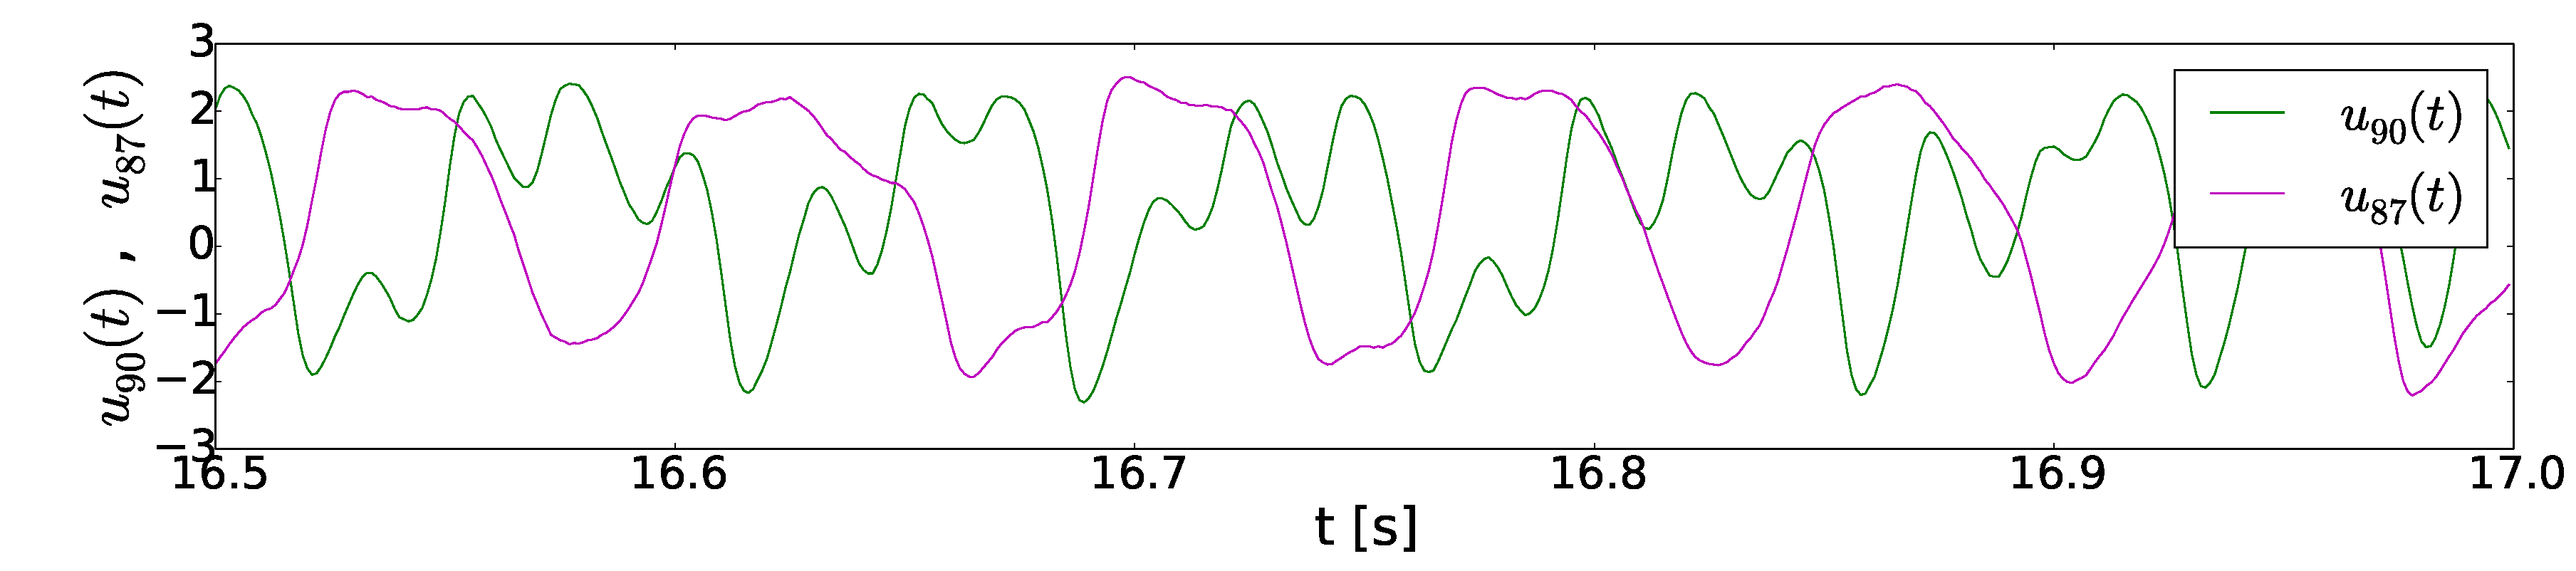
\includegraphics[width=\textwidth]{Figures/cor_FCM_sim_no_worst.eps} 

    \rule{35em}{0.5pt}
  \caption[3D Fast Fourier Transform, FHN, FCM]{3D illustration of fast fourier transform of neuronal activity oscillations corresponding to $N=90$ nodes in FCM simulation with parameters given in Fig.3.2.} 
    \label{fig:3D Fast Fourier Transform, FHN, FCM}
 	
\end{figure}  
 


\subsection{ACM Brain Graphs Compared to DW-MRI Data}

Brain graphs based on ACM are binarized via probability $p$ values between $[0.18, 0.82]$. Lower and upper $p$ in this range correspond approximately to 0.35 and 0.10 for $D$, respectively. FHN simulated ACM graphs are compared to its own empirical data derived from DW-MRI technique. Same procedures as explained in the previous section are followed while comparing simulated structural connectivity brain networks to its experimental origin.

Figure 3.5 illustrates $\rho_{e,s}$ in parameter spaces. Highest correlation regime between simulated and empirical data is captured at $4[m/s]<v<8[m/s]$, $0.1<c<0.5$ with $p<0.66$. Since network topologies in ACM based brain graphs do not change as dramatically as in FCM, larger binarization steps by amount of $0.4$ are followed here. 

Figure 3.6 indicates a correlation matrix for a simulated ACM brain graph with a high analogy to its empirical origin. The parameters are chosen in accordance with hot colored squares in Figure 3.5. Figure 3.7 demonstrates the simulated neuronal activity of the excitator variable of FHN model for two pairs of nodes, and Figure 3.8 indicates again fast oscillations arise from our model.  

\begin{figure}[htbp]
 
  \centering
    \includegraphics[width=0.49\textwidth]{Figures/PA_ACM_c_03.eps} 
	\includegraphics[width=0.49\textwidth]{Figures/PA_ACM_v_6.eps} 

	
    \rule{35em}{0.5pt}
  \caption[Parameter Analysis, ACM]{FHN simulated ACM brain graphs, parameter analysis, $v=6[m/s]$ on the left and $c=0.3$ on the right }
  \label{fig:Parameter Analysis, ACM}
 	
\end{figure} 

 
\begin{figure}[htbp]
 
  \centering
	 \includegraphics[width=0.49\textwidth]{Figures/cor_ACM_sim.eps} 
   	 \includegraphics[width=0.49\textwidth]{Figures/cor_ACM_exp.eps} 

    \rule{35em}{0.5pt}
  \caption[High correlated FHN simulation, ACM]{FHN model simulated ACM graph (on the left) and empirical DW-MRI (on the right) correlation matrices. The parameters for extracted timeseries are $c=0.3$, $v=6 [m/s]$, $r=0.50$, overall correlation between two matrices is $\rho_{e,s} = 0.43$.} 
    \label{fig:High correlated FHN simulation, ACM}
 	
\end{figure}



\begin{figure}[htbp]
 
  \centering
	 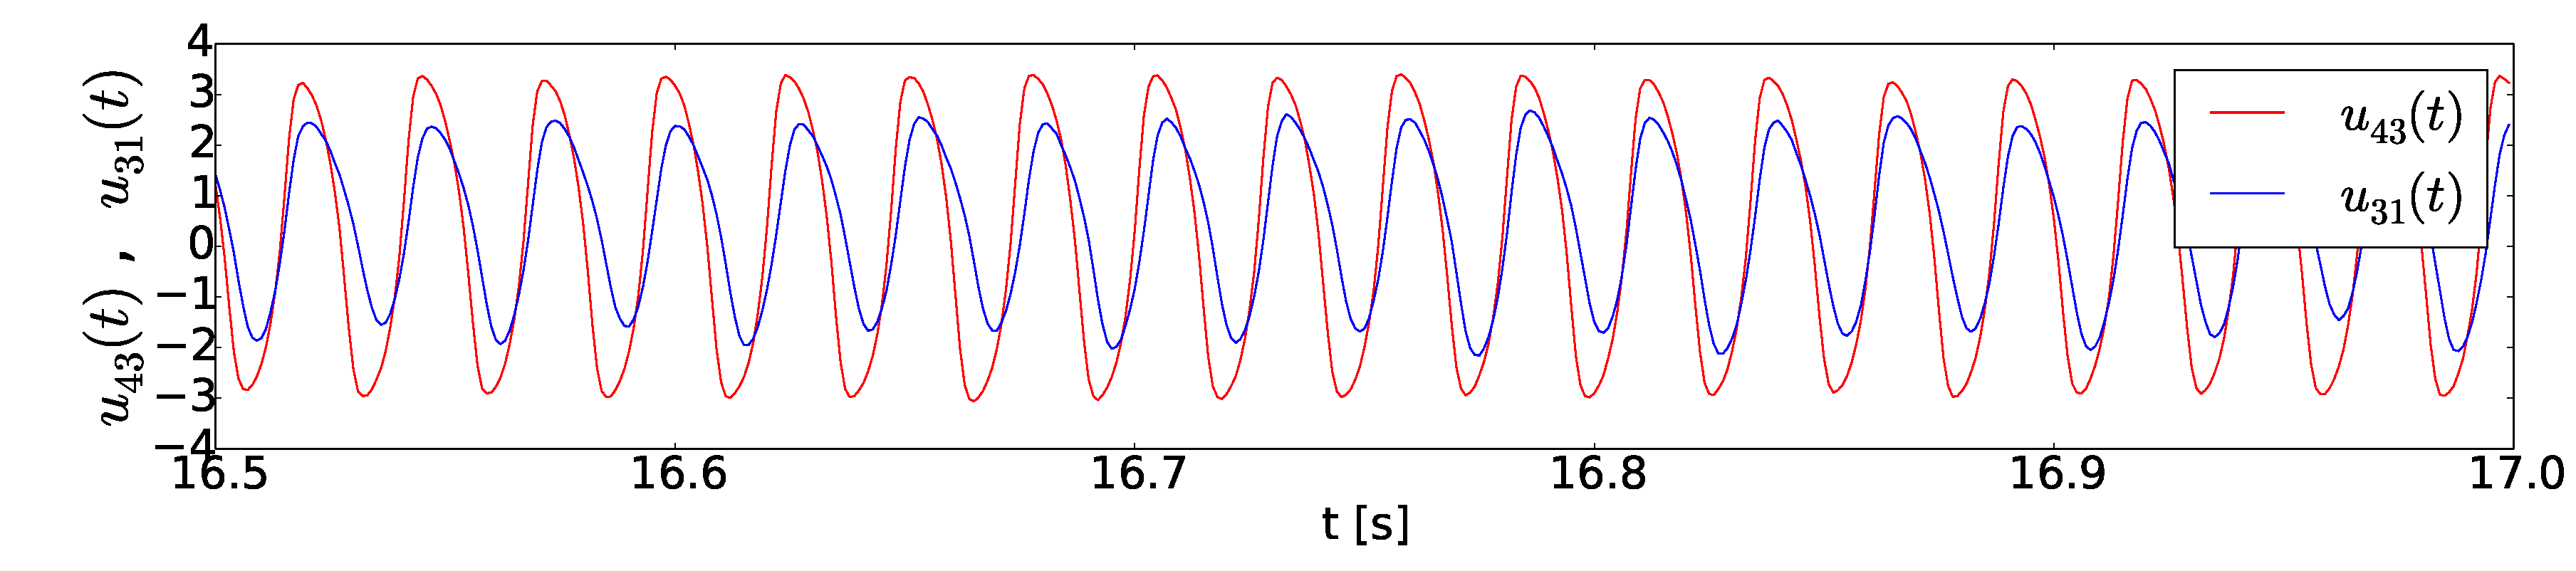
\includegraphics[width=\textwidth]{Figures/cor_ACM_sim_no_best.eps} 
   	 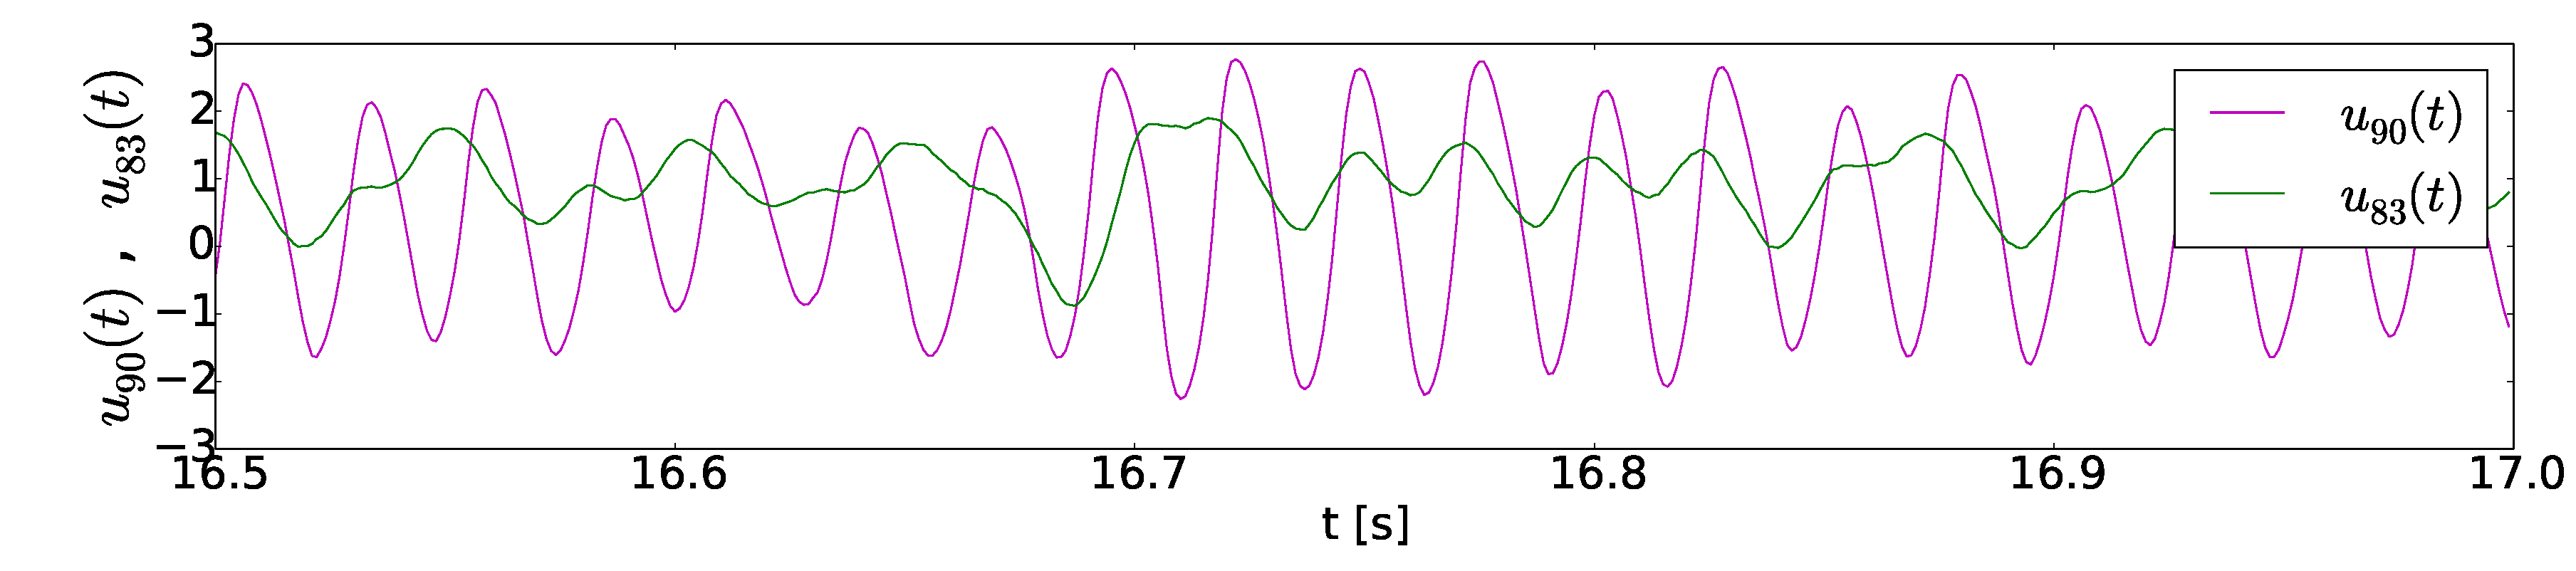
\includegraphics[width=\textwidth]{Figures/cor_ACM_sim_no_worst.eps} 

    \rule{35em}{0.5pt}
  \caption[Neural Activity Node Dynamics, ACM]{Simulated neuronal activity of highly (at top, $\rho_{43,31}=0.86$) and poorly (at bottom, $\rho_{90,83}=0.15$) correlated node couples. Both nodes are chosen from the simulated correlation matrix of ACM in previous figure ($c=0.3$, $v=6 [m/s]$, $r=0.50$).} 
    \label{fig:Neural Activity Node Dynamics, ACM}
 	
\end{figure} 




\begin{figure}[htbp]
 
  \centering
	 \includegraphics[width=0.8\textwidth]{Figures/FFT_ACM.eps} 
   	 %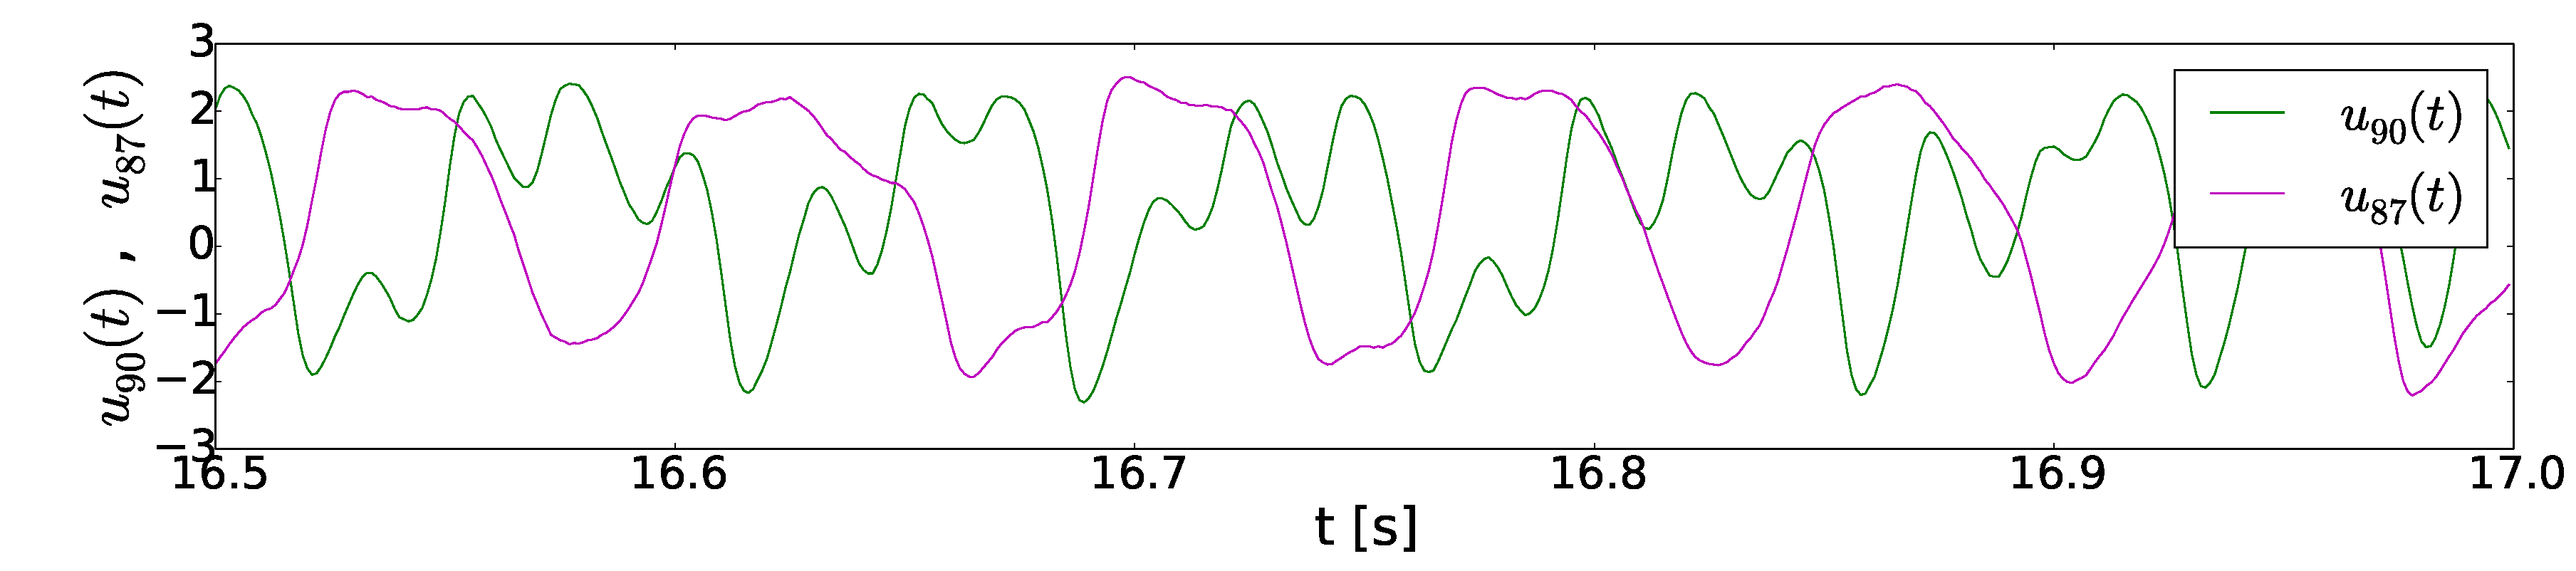
\includegraphics[width=\textwidth]{Figures/cor_FCM_sim_no_worst.eps} 

    \rule{35em}{0.5pt}
  \caption[3D Fast Fourier Transform, FHN, ACM]{3D illustration of fast fourier transform of neuronal activity oscillations corresponding to $N=90$ nodes in ACM simulation with parameters given in Fig.3.6.} 
    \label{fig:3D Fast Fourier Transform, FHN, ACM}
 	
\end{figure}  




\section{BOLD Activity Simulations}

Brain graphs based on FCM and ACM are simulated further with Balloon-Windkessel hemodynamic model in order to capture BOLD fluctuations, which is thought to be the origin of from fMRI-BOLD technique. All simulated neuronal activity oscillations are normalized around their mean, and then the BOLD activity is inferred via hemodynamics as described in section 2.6. It is already expected to produce a well correlated BOLD simulation on FCM derived brain graph as previous studies have already stated \citep{VUK13}. However, extraction of BOLD signal through structural connectivity is not yet completely clarified. This section presents any correlations between simulated BOLD activity of FCM and fMRI-BOLD, as well as that of ACM and fMRI BOLD. 

FHN temporal dynamics in parameter spaces $(c,r)$ and $(c,p)$ are further used for BOLD activity simulations, right hand sides of Figures 3.1 and 3.5 can be reviewed for FCM and ACM timeseries sources. Figure 3.9 shows comparisons between simulated and experimental BOLD correlation matrices via Pearson's statistical approach. fMRI-BOLD matrix seems to be in better agreement with FCM based simulations than that of ACM. In both cases, BOLD signal seems to  be better correlated in $c<0.2$. Small $c$ values result in better $\rho{e,s}$, which was observed oppositely in FHN simulations. The effect of binarization is more pronounced in brain graphs derived from ACM, i.e. $p<0.74$ results usually in higher $\rho{e,s}$.

Figures 3.10 and 3.13 visualize BOLD activity correlation matrices chosen from hot colored parameters in Figure 3.9. The next step is to inquire nodal BOLD fluctuations in pairs of highly and poorly correlated nodes as given in Figures 3.11 and 3.14. Lastly, Fast Fourier Transforms for all nodes in chosen simulation sets are performed. Figure 3.12 and 3.15 are limited to frequency $\nu$ between $0$ and $2[Hz]$, there is no higher $\nu$ than those values observed in BOLD activity simulations.




\begin{figure}[htbp]
 
  \centering
    \includegraphics[width=0.49\textwidth]{Figures/PA_BOLD_FCM_v_7.eps} 
	\includegraphics[width=0.49\textwidth]{Figures/PA_BOLD_ACM_v_3.eps} 

	
    \rule{35em}{0.5pt}
  \caption[Parameter Analysis, BOLD]{Parameter analysis for BOLD simulations applied on FCM (on the left, $v=7 [m/s]$) and ACM (on the right, $v=3 [m/s]$ ) obtained brain graphs compared to fMRI-BOLD data. }
  \label{fig:Parameter Analysis, BOLD}
 	
\end{figure} 



\begin{figure}[htbp]
 
  \centering
	 \includegraphics[width=0.49\textwidth]{Figures/cor_BOLD_FCM_sim.eps} 
   	 \includegraphics[width=0.49\textwidth]{Figures/cor_FCM_exp.eps} 

    \rule{35em}{0.5pt}
  \caption[High correlated BOLD simulation, FCM]{Highly correlated BOLD simulation of FCM brain graph with $c=0.03$, $v=7 [m/s]$ and $r=0.66$ (on the left) and fMRI-BOLD data, $\rho_{e,s} = 0.24$.} 
    \label{fig:High correlated BOLD simulation, FCM}
 	
\end{figure}  





\begin{figure}[htbp]
 
  \centering
	 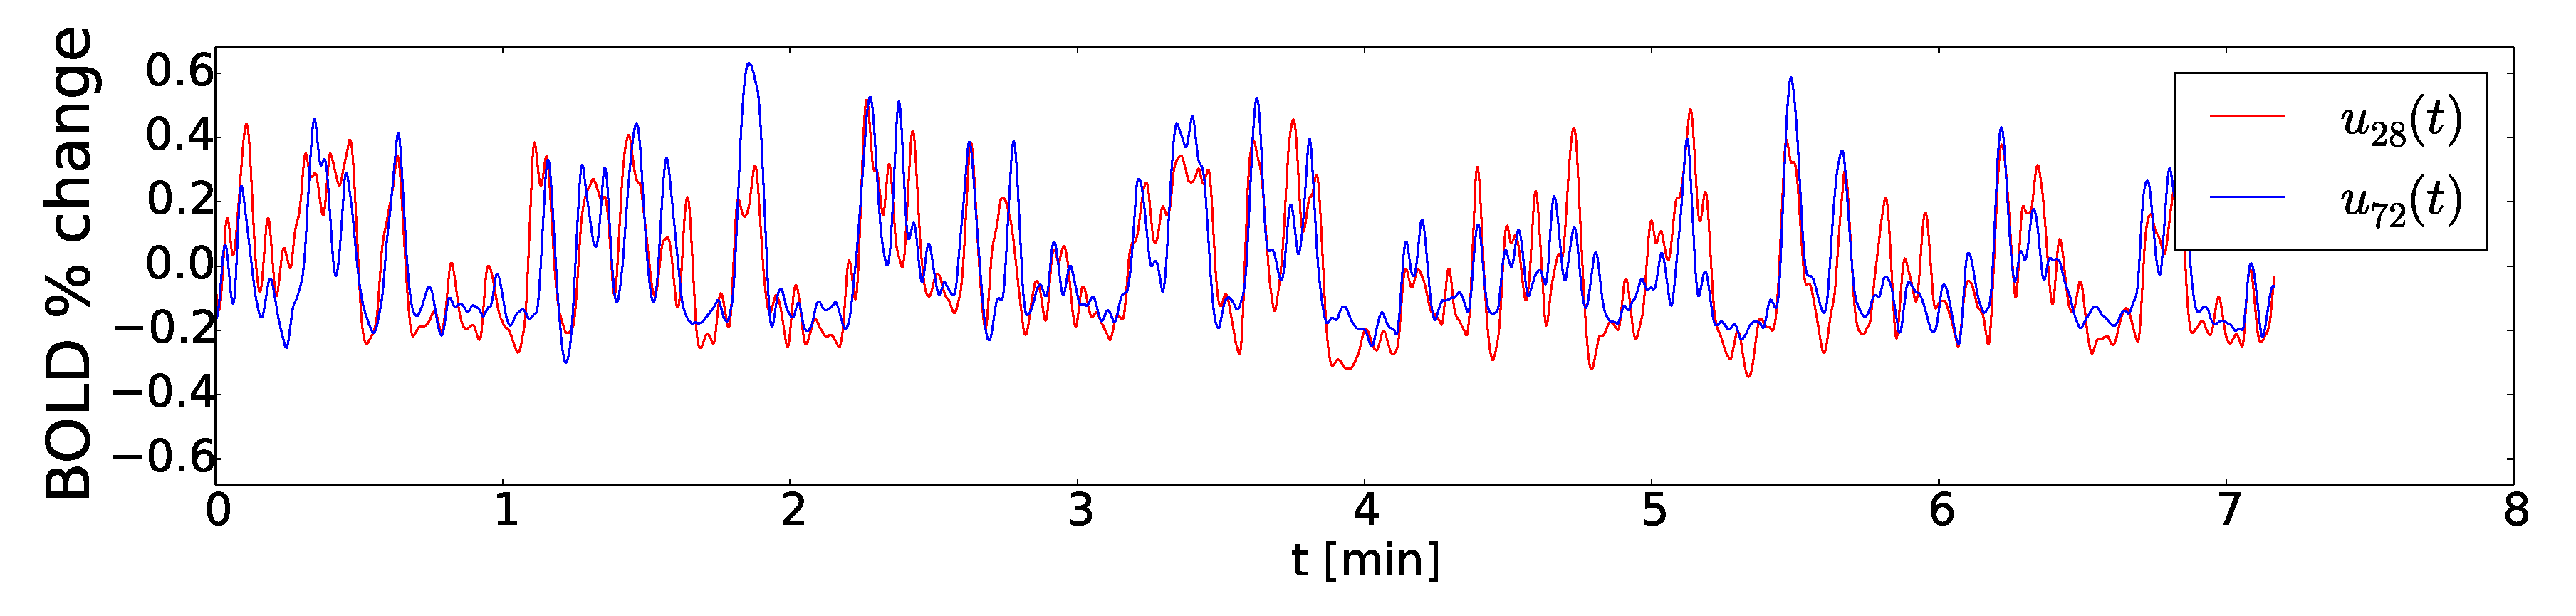
\includegraphics[width=\textwidth]{Figures/cor_BOLD_FCM_sim_no_best.eps} 
   	 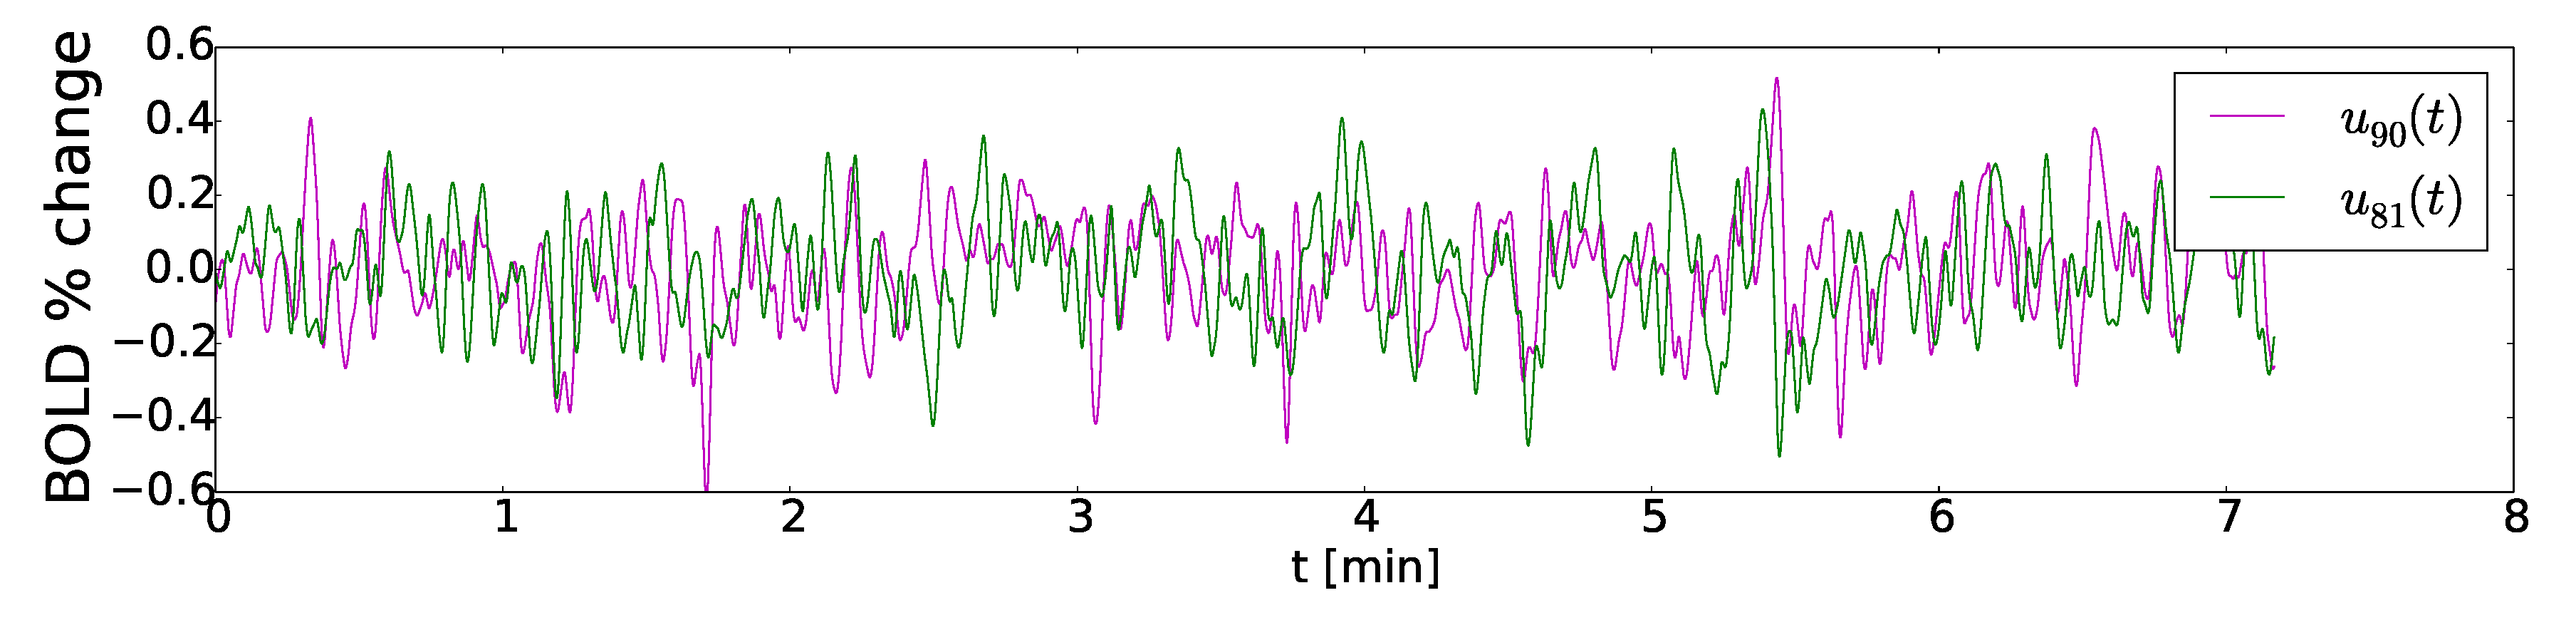
\includegraphics[width=\textwidth]{Figures/cor_BOLD_FCM_sim_no_worst.eps} 

    \rule{35em}{0.5pt}
  \caption[BOLD Activity Node Dynamics, FCM]{Simulated BOLD activity of highly (at top, $\rho_{28,72}=0.75$) and poorly (at bottom, $\rho_{90,81}=0.11$) correlated node couples. Both nodes are chosen from the simulated correlation matrix in previous figure ($c=0.03$, $v=7 [m/s]$, $r=0.66$).} 
    \label{fig:BOLD Activity Node Dynamics, FCM}
 	
\end{figure} 



\begin{figure}[htbp]
 
  \centering
	 \includegraphics[width=0.8\textwidth]{Figures/FFT_BOLD_FCM.eps} 
   	 %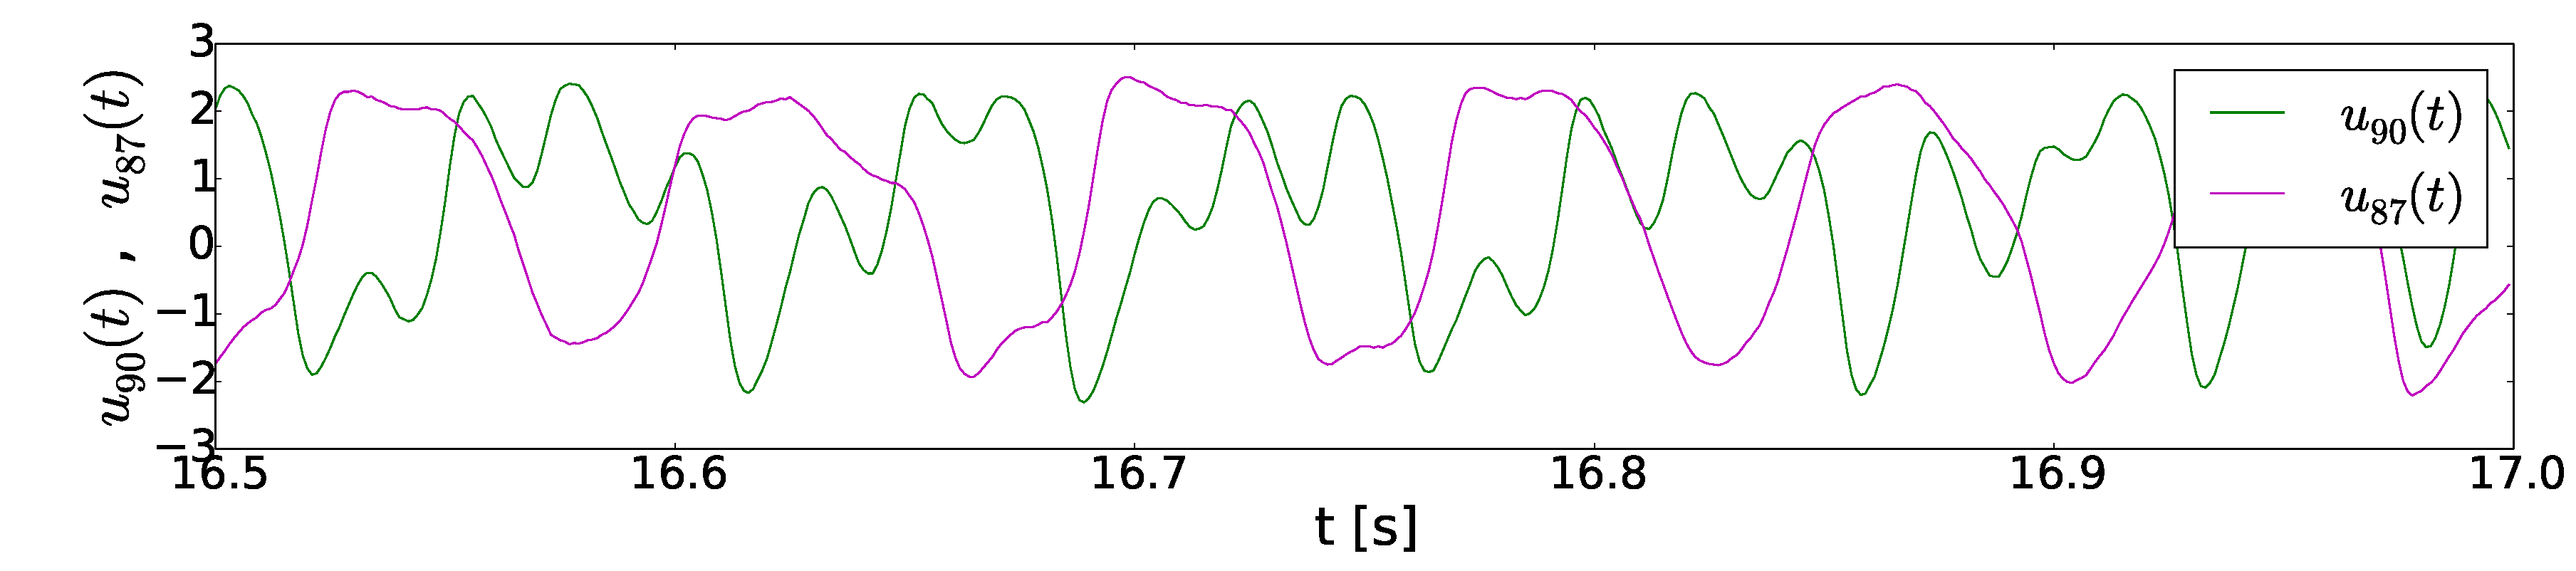
\includegraphics[width=\textwidth]{Figures/cor_FCM_sim_no_worst.eps} 

    \rule{35em}{0.5pt}
  \caption[3D Fast Fourier Transform, BOLD, FCM]{3D illustration of fast fourier transform of BOLD activity slow oscillations corresponding to $N=90$ nodes in FCM simulation with parameters given in Fig.3.10.} 
    \label{fig:3D Fast Fourier Transform, BOLD, FCM}
 	
\end{figure}  


\begin{figure}[htbp]
 
  \centering
	 \includegraphics[width=0.49\textwidth]{Figures/cor_BOLD_ACM_sim.eps} 
   	 \includegraphics[width=0.49\textwidth]{Figures/cor_FCM_exp.eps} 

    \rule{35em}{0.5pt}
  \caption[High correlated BOLD simulation, ACM]{Highly correlated BOLD simulation of ACM brain graph with $c=0.03$, $v=3 [m/s]$ and $r=0.54$ (on the left) and empirical FCM obtained from fMRI-BOLD. $\rho_{e,s} = 0.22$} 
    \label{fig:High correlated BOLD simulation, ACM}
 	
\end{figure}  




\begin{figure}[htbp]
 
  \centering
	 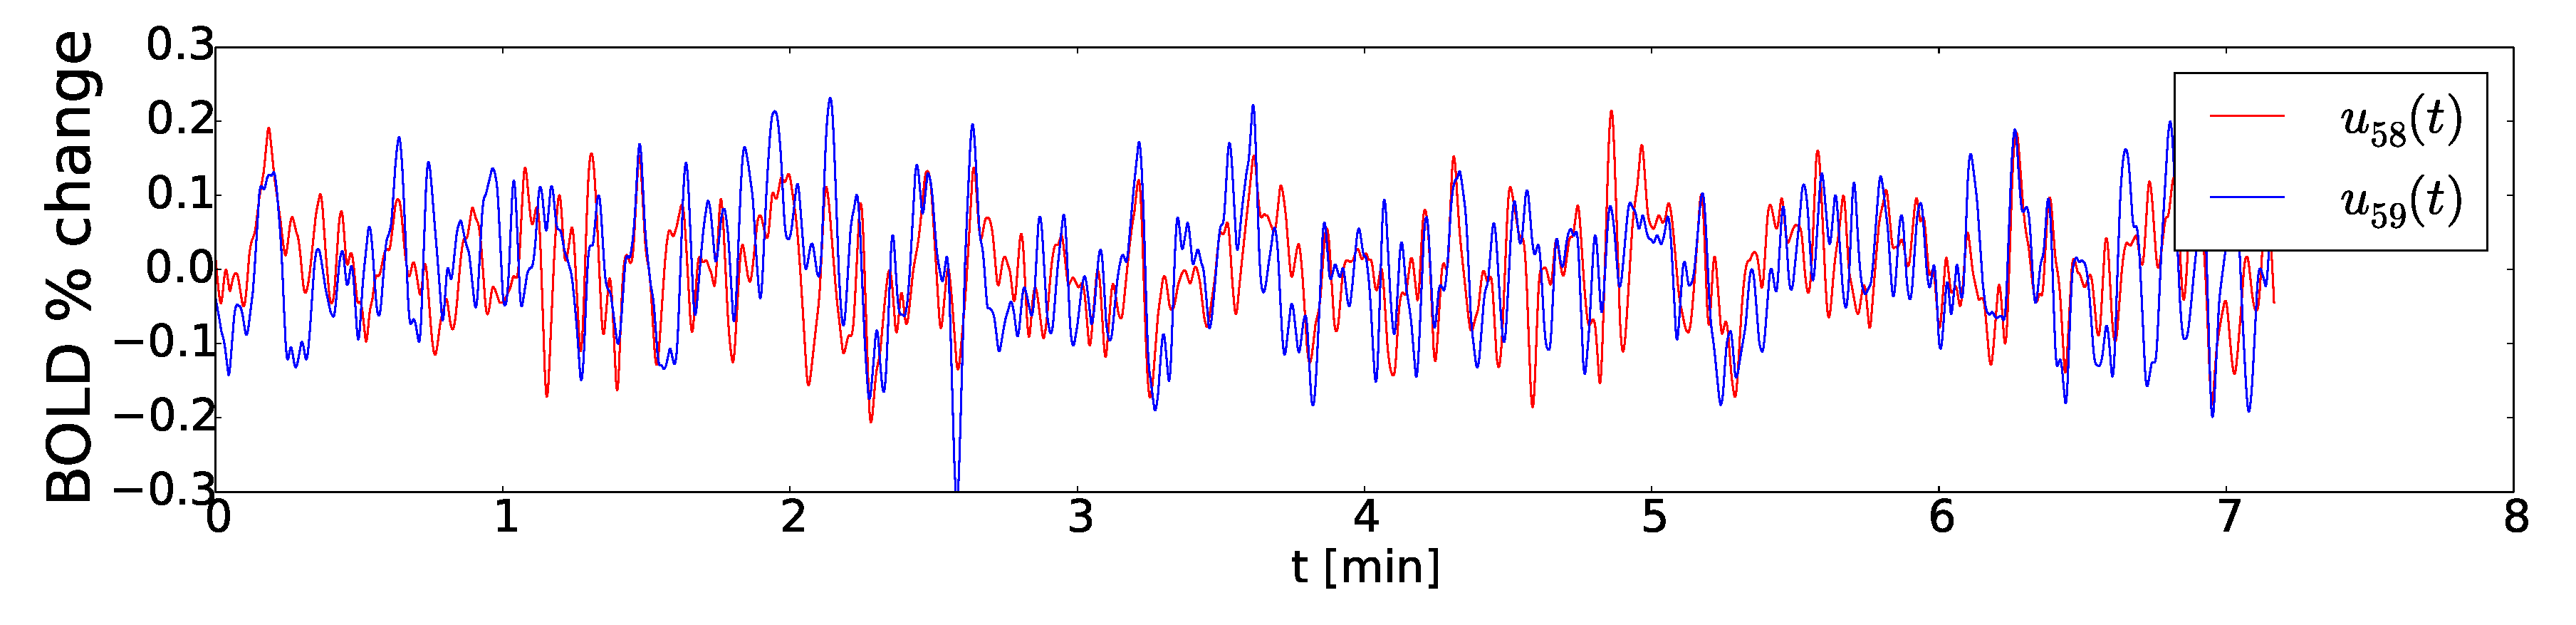
\includegraphics[width=\textwidth]{Figures/cor_BOLD_ACM_sim_no_best.eps} 
   	 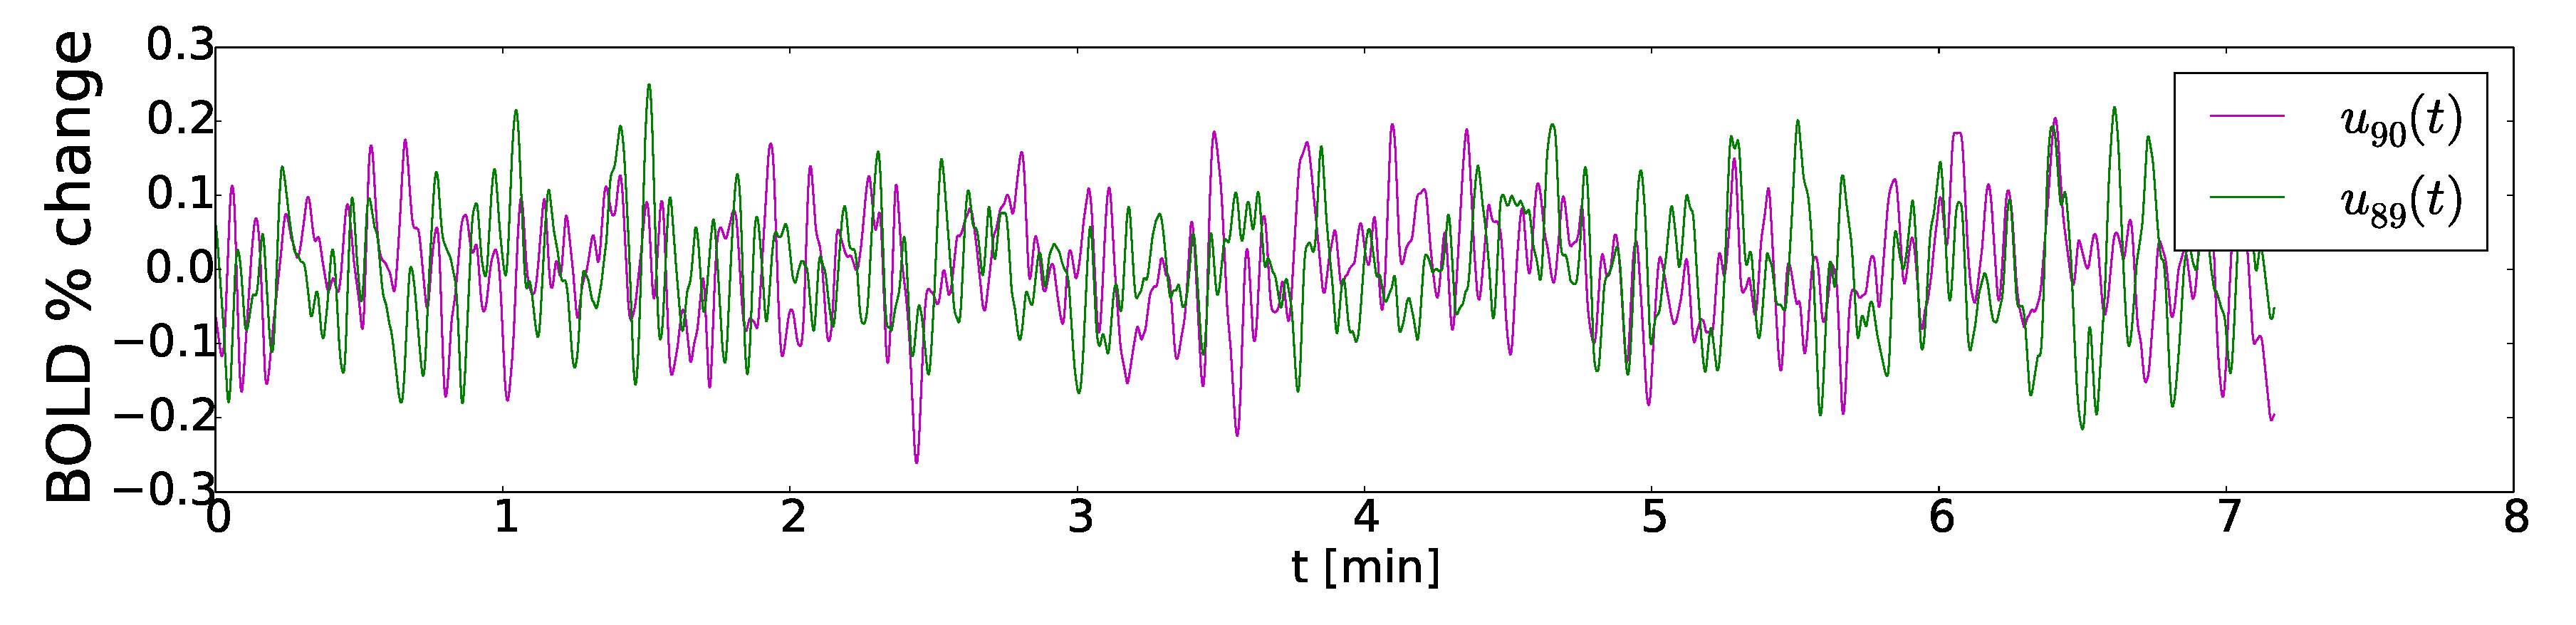
\includegraphics[width=\textwidth]{Figures/cor_BOLD_ACM_sim_no_worst.eps} 

    \rule{35em}{0.5pt}
  \caption[BOLD Activity Node Dynamics, ACM]{Simulated BOLD activity of highly (at top, $\rho_{58,59}=0.48$) and poorly (at bottom, $\rho_{90,89}=0.11$) correlated node couples. Both nodes are chosen from the simulated ACM correlation matrix in previous figure ($c=0.03$, $v=3 [m/s]$, $r=0.54$).} 
    \label{fig:BOLD Activity Node Dynamics, ACM}
 	
\end{figure} 






\begin{figure}[htbp]
 
  \centering
	 \includegraphics[width=0.49\textwidth]{Figures/FFT_BOLD_FCM.eps} 
   	 %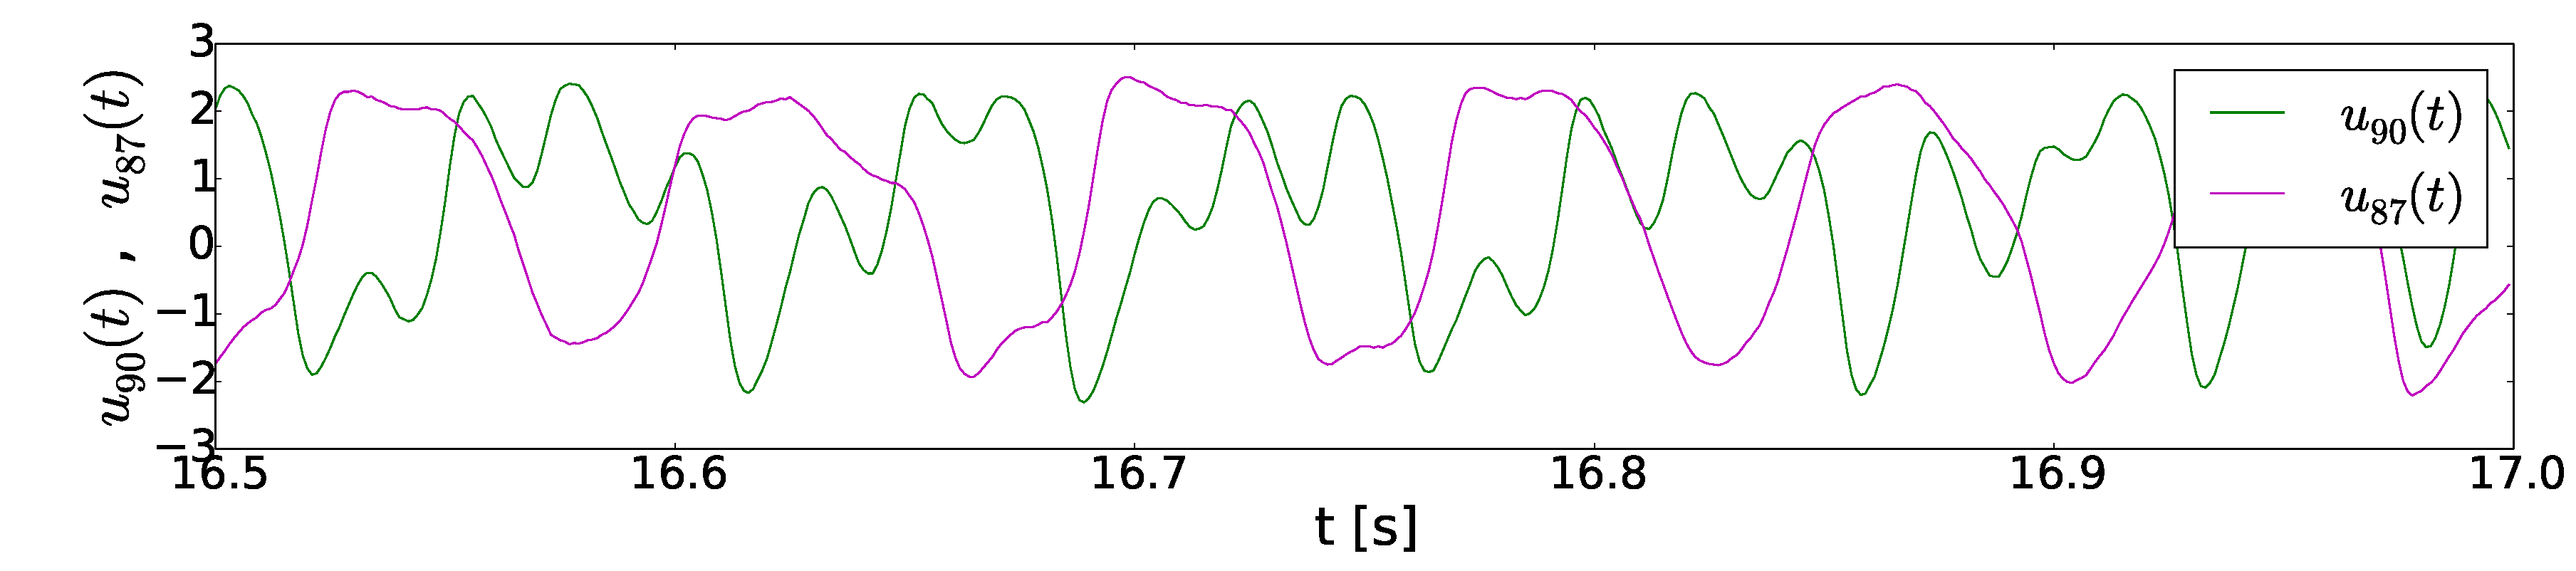
\includegraphics[width=\textwidth]{Figures/cor_FCM_sim_no_worst.eps} 

    \rule{35em}{0.5pt}
  \caption[3D Fast Fourier Transform, BOLD, ACM]{3D illustration of fast fourier transform of BOLD activity slow oscillations corresponding to $N=90$ nodes in ACM simulation with parameters given in Fig.3.13.} 
    \label{fig:3D Fast Fourier Transform, BOLD, ACM}
 	
\end{figure}  

\clearpage

\section{Comparison of Brain Graph to Random Graphs}


All randomly constructed brain graphs are simulated with FHN model for the same $r$ and $c$ used for brain graph neuronal activity simulations. The correlation coefficient between all possible node pairs is calculated via Pearsons correlation coefficient $\rho_{ij}$ and all $\rho$ values are distributed in histogram plots as seen in Figure 3.16. The FHN time-series of the nodes in the brain graph simulation seems to be uniformly distributed around no correlation $\rho=0$. The time-series extracted from random graphs tend to dominate around high correlations and anti-correlations. 



\begin{figure}[htbp]
 
  \centering
	 \includegraphics[width=\textwidth]{Figures/Random_FCM_histo.eps}
  \caption[Histogram Comparison, FCM]{Histogram for the distribution of Pearson correlations among all possible pairwise combinations of nodes, $\rho_{i,j}$ in FHN simulated brain graphs and random graphs (on the left, from top to bottom : $R0$, $Rd$, $Rh$, on the right, from top to bottom: $Ra$, $Rg$, $Rk$). } 
    \label{fig:Histogram Comparison, FCM}
 	
\end{figure}  

\begin{figure}[htbp]
 
  \centering
	 \includegraphics[width=\textwidth]{Figures/Random_FCM_PA.eps}
  \caption[Random Graph Comparison, FCM]{Each heat map corresponds to statistical comparison of brain graph to random graphs, (on the left, from top to bottom : $Ra$, $Rg$, $Rh$, on the right, from top to bottom: $Rd$, $Rk$). The FHN model parameters are $r=61$, $v=7[m/s]$ and $c=0.1$. Colorbars present Bhattacharya coefficients $d(H_r, H_b)$. } 
    \label{fig:Random Graph Comparison, FCM}
 	
\end{figure}  

Histogram distribution of Pearson correlation coefficients between all possible node pairs is further used to compare brain graphs to random networks. Figure 3.17. represents if brain graphs are distinguishable than random graphs in parameter space $(r,c)$ with Bhattacharya coefficients $d(H_r, H_b)$. The hot colors indicate diversity, whereas the cold colors denote analogy. It can be inferred that brain graph simulations become can be distinguished from random graph simulations in terms of modeled neuronal activity at low coupling strengths $c<0.2$ in general.   The parameters of previous figure is already chosen with the help of hot colored $d(H_r, H_b)$ in Figure 3.17 to demonstrate diversity.


TO DO : BOLD SIMULATIONS ON A-AAL RANDOM GRAPHS IN FIGURE 3.17 , FHN SIMULATIONS ON ACP-W RANDOM GRAPHS, BOLD SIMULATIONS ON ACP-W RANDOM GRAPHS !



